\documentclass[11pt, oneside]{article}   	% use "amsart" instead of "article" for AMSLaTeX format
\usepackage{geometry}                		% See geometry.pdf to learn the layout options. There are lots.
\geometry{letterpaper}                   		% ... or a4paper or a5paper or ... 
%\geometry{landscape}                		% Activate for rotated page geometry
%\usepackage[parfill]{parskip}    		% Activate to begin paragraphs with an empty line rather than an indent
\usepackage{graphicx}				% Use pdf, png, jpg, or eps§ with pdflatex; use eps in DVI mode
								% TeX will automatically convert eps --> pdf in pdflatex		
\usepackage{amssymb}
\usepackage{verbatim}
\usepackage{url}


\setlength{\parskip}{1ex} %--skip lines between paragraphs
\setlength{\parindent}{0pt} %--don't indent paragraphs

\title{
	Vulnerability Report for\\
	OHNO PTE. LTD.
}
\author{
	prepared by\\
	JOSEPH MATTHIAS GOH\\
	OHYES SECURITY PTE. LTD.
}
\date{on 15/12/2016}
\begin{document}

\maketitle
\newpage

\tableofcontents
\newpage

\section{Executive Summary}
OHNO PTE LTD has indicated unusual behaviour on a machine
with a Windows 7 Enterprise operating system installed. The machine
in question is being used as a local continuous integration (CI) server
for their primary product, Nobuty, and is used to run regression tests 24/7.\\

Due to a new company policy on being able to access their CI server from
anywhere in the world, the development team has disabled the default
firewall one year ago but have only recently noticed that the machine
shuts down at random times of the day, and the technical lead suspects
that the machine has been compromised by hackers. The machine has since
been isolated together with another machine that acts as a backup. Both
machines are on the same network.\\

OHYES SECURITY has been tasked with doing a general scan of OHNO's 
networks and to provide recommendations on possible courses of action
to the management team.

\section{Service Agreement Overview}
\subsection{Summary}
OHYES SECURITY will perform an Internal Network Vulnerability Assessment
for up to 255 local network IP addresses on a single network with the goal
of validating suspected vulnerabilities in OHNO PTE LTD's 
computing infrastructure. Services will be performed on-site in the 
presence of a project manager assigned by OHNO PTE LTD.\\

The engagement period was agreed to be between 12th December 2016 to 31st December 2016.

\subsection{Vendor Responsibilities}
\begin{itemize}
\item{
	Conduct a scan on the network to confirm the number of computers
	on the network for up to 255 local network addresses.
}
\item{
	Identify the offending computer identified by Asset Tag No.
	XCAON-18553231-A running Windows 7 Enterprise and perform
	a vulnerability scan on it.
}
\item {
	Perform data correation by researching on vulnerabilities,
	eliminating false positives where possible, investigating
	the potential impact of the findings, and providing recommended
	remediations.
}
\item{
	Provide Customer with a Machine Vulnerability Assessment Report.
}
\end{itemize}
\subsection{Customer Responsibilities}
\begin{itemize}
\item {
	Identify an on-site project manager to assist in coordinating 
	Customer's resource(s).
}
\item{
	Provide OHYES SECURITY with access to the business site during
	Standard Business Hours including buildings, parking, phone systems,
	internet access, server rooms and workstations.
}
\item{
	Provide OHYES SECURITY with access to a suitable conference room 
	facility for mettings, interviews and facilitated sessions during 
	the engagement period.
}
\item{
	Provide physical and wireless access to the offending network
}
\item{
	Provide access to available resources related to the business
	and technical environment including operating systems, network
	and any computing environments necessary for OHYES SECURITY to
	complete the Services.
}
\item{
	Review with OHYES SECURITY the completed Assessment Report
}
\item{
	Provide sign-off for completed Machine Vulnerability Assessement
	services.
}

\end{itemize}

\subsection{Waiver of Liability}
\begin{itemize}
\item{
	Customer understands and acknowledges that where OHYES SECURITY has
	exercised reasonable precautions in delivering the Service, OHYES
	SECURITY is not responsible for system outages, degradation of
	performance or other adverse technology environment consequences of
	tasks Customer has authorised OHYES SECURITY to perform.
}
\item{
	Customer represents and warrant that they have sufficient authroity and
	the rights necessary for Customer to provide and/or facilitiate OHYES 
	SECURITY's access to information, data, networks, systems, and media in
	connection with these SErvices.
}
\item{
	For all Customer requests under this Service Agreement that OHYES SECURITY
	posses, access, or analyze particular media, computers, computer networks,
	communications networks, or other systems and equipment, to the extent
	Customer provides or facilitates Cisco's access thereto. Customer
	represents, warrants and covenants that they have all necessary right, 
	title, license and autrhoity to make such requests and grant such access, 
	including permissions from third-party owners of licensed or shared resources.
}
\item{
	Any delays in provision of necessary test access, environments, VPN 
	connections, user accounts, administrative access, or other required 
	technical assets may result in delay of deliverables and/or reduction of 
	the scope of work performed.
}
\item {
	Customer acknowledges that the completion of Services is dependent upon 
	Customer meeting its responsibilities as indicated herein.
}
\item {
	Customer will identify Customer's personnel and define their roles in the 
	participation of the Services. Such personnel may include but is not limited 
	to: architecture design and planning engineers, and network engineers.
}
\item {
	Customer will ensure Customers's personnel are available to participate during 
	the course of the Services to provide information and to participate in the 
	scheduled information gathering sessions, interviews, meetings and conference 
	calls.
}
\item {
	Customer expressly understands and agrees that support services provided by 
	OHYES SECURITY comprise technical advice, assistance and guidance only.
}
\item {
	Customer understands that any IP addresses not utilised during the term of 
	the Service will not result in any credit.
}
\item {
	Customer expressly understands and agrees that the Services shall take place 
	and complete within fifty (50) calendar days from issuing a Purchase Order to 
	OHYES SECURITY for the Services herin and any unused hours will expire.
}
\end{itemize}

\subsection{Costing}
OHNO PTE LTD has agreed to pay OHYES SECURITY SGD \$10,000.00 for the
afore-describe service.

\section{Methodology}

\subsection{Tools}
The following section specifies tools that will be used.

\subsubsection{NMap}
Nmap\footnote{Related Link: \url{https://nmap.org/}} is a free and open 
source utility for network discovery and security auditing. \\

Nmap uses raw IP packets to determine available hosts on a network, what services those
hosts are offering, what operating systems they are running, and what type of firewalls are
in place among other functionalities.


\subsubsection{ZenMap}
ZenMap\footnote{Related Link: https://nmap.org/zenmap/} is an open-source cross-platform
graphical user interface for Nmap which we use to visualise the network.

\subsubsection{Nessus}
Nessus\footnote{Related Link: https://www.tenable.com/products/nessus-vulnerability-scanner} 
is a proprietary vulnerability scanner created by Tenable Network Security. \\

Related Link: https://www.tenable.com/products/nessus-vulnerability-scanner

\subsection{Process}

\begin{enumerate}
\item{Host Discovery}
\subitem{
	We proceed by first scanning the network using Nmap to confirm the number of hosts. 
}
\item{Host Isolation}
\subitem{
	A port scan will be run to determine likelihood of vulnerabilities. A service scan will
	also be run to determine the likelihood of a computer having vulnerabilities.
}
\item{Risk Management}
\subitem{
	A visulisation of the network topology will be generated to understand other hosts and
	identify potential risks in performing a vulnerability scan on the network.
}
\item{Vulnerability Scanning}
\subitem{
	After identification of the offending host, we use Nessus to run a vulnerability scan on it
	to determine exact vulnerabilities which we will generate remdiation steps from.
}
\end{enumerate}

\section{Information Gathering}
\subsection{Nmap Command}
\begin{figure}[h!]
	\fontsize{10pt}{8pt}
	\begin{verbatim}
	nmap -T4 -A -vv -Pn 192.168.108.15
	\end{verbatim}}
	\caption{Nmap command used for gathering information about the network}
\end{figure}

\subsection{Machines on Network}
The scan discovered two hosts, 192.168.108.15 and 192.168.108.88, with 
a large number of open ports on 192.168.108.15 and none on 192.168.108.88.\\

\begin{figure}[h!]
	\fontsize{8pt}{4pt}
	\begin{verbatim}
...

Initiating SYN Stealth Scan at 20:40
Scanning 2 hosts [1000 ports/host]
Completed SYN Stealth Scan against 192.168.108.88 in 8.03s (1 host left)
Discovered open port 49157/tcp on 192.168.108.15
Discovered open port 2103/tcp on 192.168.108.15
Increasing send delay for 192.168.108.15 from 0 to 5 due to 11 out of 11 dropped probes since last increase.
Increasing send delay for 192.168.108.15 from 5 to 10 due to 11 out of 12 dropped probes since last increase.
Discovered open port 49152/tcp on 192.168.108.15
Discovered open port 5357/tcp on 192.168.108.15
Discovered open port 9/tcp on 192.168.108.15
Discovered open port 10243/tcp on 192.168.108.15
Discovered open port 17/tcp on 192.168.108.15
Discovered open port 13/tcp on 192.168.108.15
Discovered open port 49158/tcp on 192.168.108.15
Discovered open port 19/tcp on 192.168.108.15
Discovered open port 7/tcp on 192.168.108.15
Discovered open port 2869/tcp on 192.168.108.15
Discovered open port 49153/tcp on 192.168.108.15
Discovered open port 49155/tcp on 192.168.108.15
Discovered open port 49154/tcp on 192.168.108.15
Discovered open port 2107/tcp on 192.168.108.15
Discovered open port 2105/tcp on 192.168.108.15
Discovered open port 49156/tcp on 192.168.108.15
Discovered open port 135/tcp on 192.168.108.15
Discovered open port 21/tcp on 192.168.108.15
Discovered open port 554/tcp on 192.168.108.15
Discovered open port 3389/tcp on 192.168.108.15
Discovered open port 139/tcp on 192.168.108.15
Discovered open port 445/tcp on 192.168.108.15
Discovered open port 80/tcp on 192.168.108.15
Completed SYN Stealth Scan at 20:40, 37.51s elapsed (2000 total ports)

...
	\end{verbatim}
	\caption{Host Discovery}
\end{figure}

A network topology graph was generated using Nmap to visualise machines on the network as shown
below in Figure 3.

\begin{figure}[h!]
	\centering
	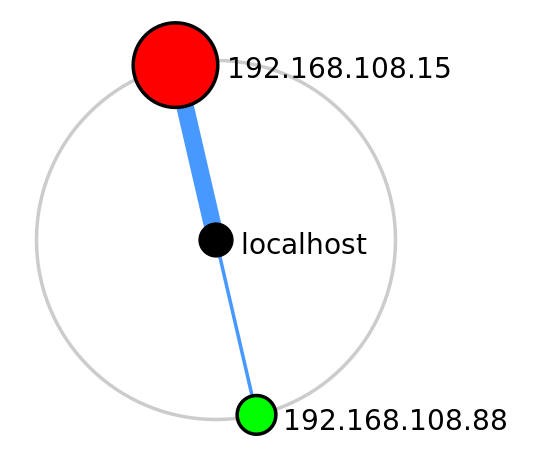
\includegraphics[width=200px]{network.png}
	\caption{Network graph}
	\label{NetworkGraph}
\end{figure}

\subsection{Host Services}

The service scan on 192.168.108.88 revealed the following host services:

\begin{figure}[h!!]
	\fontsize{8pt}{4pt}
	\begin{verbatim}
...

PORT      STATE SERVICE       VERSION
7/tcp     open  echo
9/tcp     open  discard?
13/tcp    open  daytime       Microsoft Windows USA daytime
17/tcp    open  qotd          Windows qotd (English)
19/tcp    open  chargen
21/tcp    open  ftp           FileZilla ftpd 0.9.30 beta
80/tcp    open  http          Microsoft IIS httpd 7.5
135/tcp   open  msrpc         Microsoft Windows RPC
139/tcp   open  netbios-ssn   Microsoft Windows netbios-ssn
445/tcp   open  microsoft-ds  Windows 7 Enterprise 7601 Service Pack 1 microsoft-ds (workgroup: WORKGROUP)
554/tcp   open  rtsp?
2103/tcp  open  msrpc         Microsoft Windows RPC
2105/tcp  open  msrpc         Microsoft Windows RPC
2107/tcp  open  msrpc         Microsoft Windows RPC
2869/tcp  open  http          Microsoft HTTPAPI httpd 2.0 (SSDP/UPnP)
3389/tcp  open  ms-wbt-server Microsoft Terminal Service
5357/tcp  open  http          Microsoft HTTPAPI httpd 2.0 (SSDP/UPnP)
10243/tcp open  http          Microsoft HTTPAPI httpd 2.0 (SSDP/UPnP)
49152/tcp open  msrpc         Microsoft Windows RPC
49153/tcp open  msrpc         Microsoft Windows RPC
49154/tcp open  msrpc         Microsoft Windows RPC
49155/tcp open  msrpc         Microsoft Windows RPC
49156/tcp open  msrpc         Microsoft Windows RPC
49157/tcp open  msrpc         Microsoft Windows RPC
49158/tcp open  msrpc         Microsoft Windows RPC
...
	\end{verbatim}
	\caption{Port service discovery results}
\end{figure}

\subsection{Miscellaneous Information}
The machine at 192.168.108.15 was identified with the following information which was 
in line with data provided by OHNO PTE LTD on the affected machine.
\begin{figure}[h!]
	\fontsize{8pt}{4pt}
	\begin{verbatim}
MAC Address: 08:00:27:FF:21:6D (Oracle VirtualBox virtual NIC)
Device type: general purpose
Running: Microsoft Windows 7|2008|8.1
OS CPE: cpe:/o:microsoft:windows_7::-\
	cpe:/o:microsoft:windows_7::sp1\
	cpe:/o:microsoft:windows_server_2008::sp1\
	cpe:/o:microsoft:windows_8\
	cpe:/o:microsoft:windows_8.1\
OS details: Microsoft Windows 7 SP0 - SP1, Windows Server 2008 SP1, Windows 8, or Windows 8.1 Update 1
Uptime guess: 0.602 days (since Mon Dec 19 06:18:05 2016)
Network Distance: 1 hop
TCP Sequence Prediction: Difficulty=261 (Good luck!)
IP ID Sequence Generation: Incremental
Service Info: Host: IE10WIN7; OS: Windows; CPE: cpe:/o:microsoft:windows
	\end{verbatim}
	\caption{Device details}
\end{figure}

\section{Vulnerability Scan}
A custom policy using all available Plugins and Compliance Checks was used because
no information about the underlying network infrastructure has been made known to us.\\





ARP, TCP and ICMP pings were used.

\begin{figure}[h!]
	\centering
	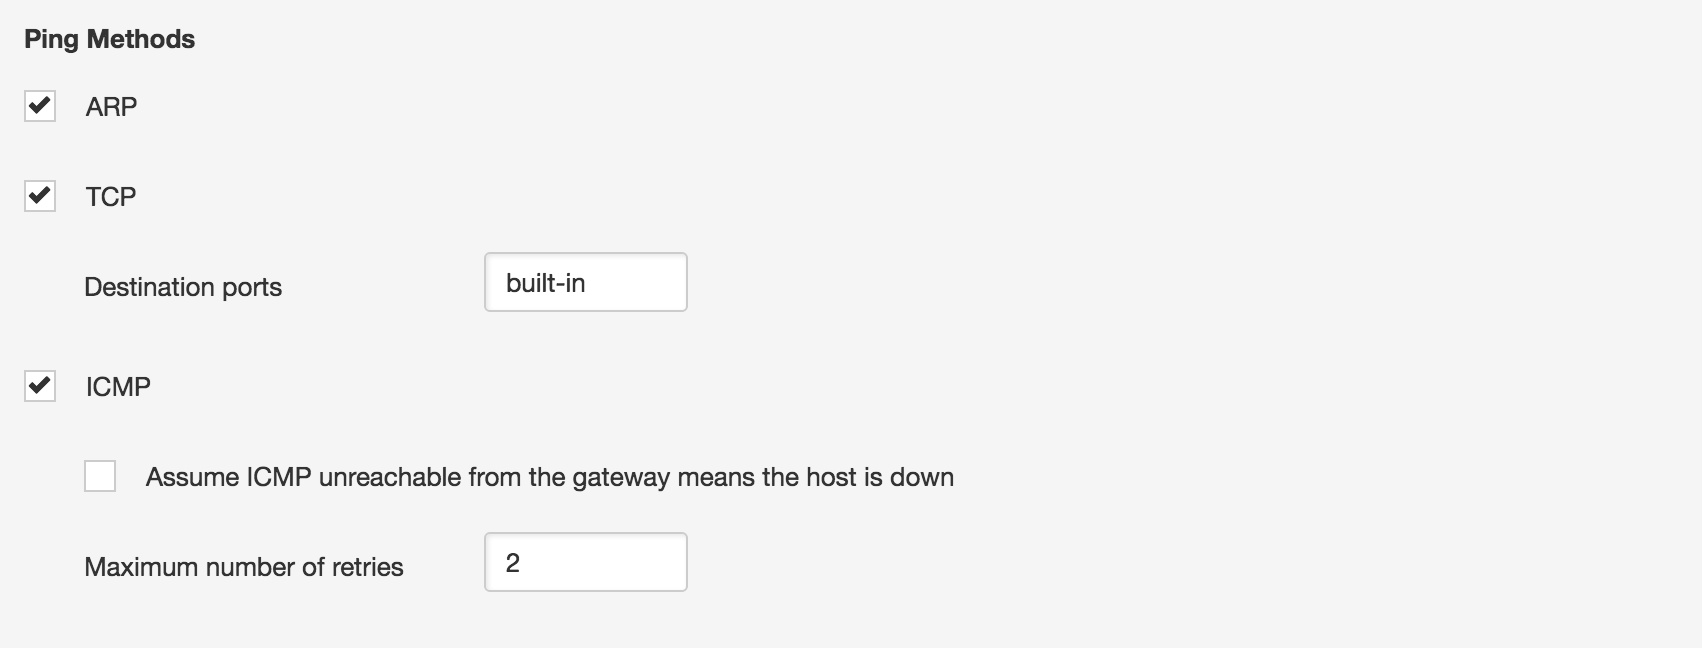
\includegraphics[width=380pt]{ping-methods.png}
	\caption{Network graph}
	\label{NetworkGraph}
\end{figure}


\section{Remediations}
\appendix
\section{Appendix}
\subsection{Service Agreement}

\end{document}  